\section{CalibX标定系统}
CalibX标定系统由软件系统和硬件系统组成。
\subsection{硬件}
硬件系统如图\ref{moon2_device}所示。该硬件系统主要由机械臂、标定板、光源、计算机及显示器、供电系统等组成。
\begin{figure}[h]
	\centering
	\includegraphics[width=1\textwidth]{figure/cp10/moon2_device}
	\caption{CalibX硬件系统}
	\label{moon2_device}
\end{figure}
该系统具有如下优点:
\begin{itemize}
	\item 立体标定板,支持大FOV鱼眼相机、支持多相机,多相机之间可以无重叠视场
	\item 4向可调高亮高均匀光源,箱体内镜头处光源强度可达2000lux,降低相机曝光时间,减轻卷帘曝光影响
	\item 机械臂、滑台滑环组合,连续转动不绕线
\end{itemize}
一些标定样品如图\ref{fig:calibx}所示。
\begin{figure}
	\centering
	\begin{minipage}{0.45\linewidth}
		\centering
		\subfigure[标定手机]{\includegraphics[width=\linewidth,height=8cm]{figure/cp10/cellphone}}
		\label{fig:subcaption1}
	\end{minipage}\qquad
	\begin{minipage}{0.45\linewidth}
		\centering
		\subfigure[标定眼镜]{\includegraphics[width=\linewidth,height=8cm]{figure/cp10/ar_glass}}
		\label{fig:subcaption2}
	\end{minipage}
	\caption{CalibX标定系统标定产品样例}
	\label{fig:calibx}
\end{figure}
\subsection{软件}
软件系统如图\ref{fig:calibx_framework}所示。整个标定系统主要包含四个模块:IMU噪声标定、静态相机标定、卷帘(rolling shutter,简称RS)RS标定和Visual-Inertial(VI)联标。
\begin{figure}[h]
	\centering
	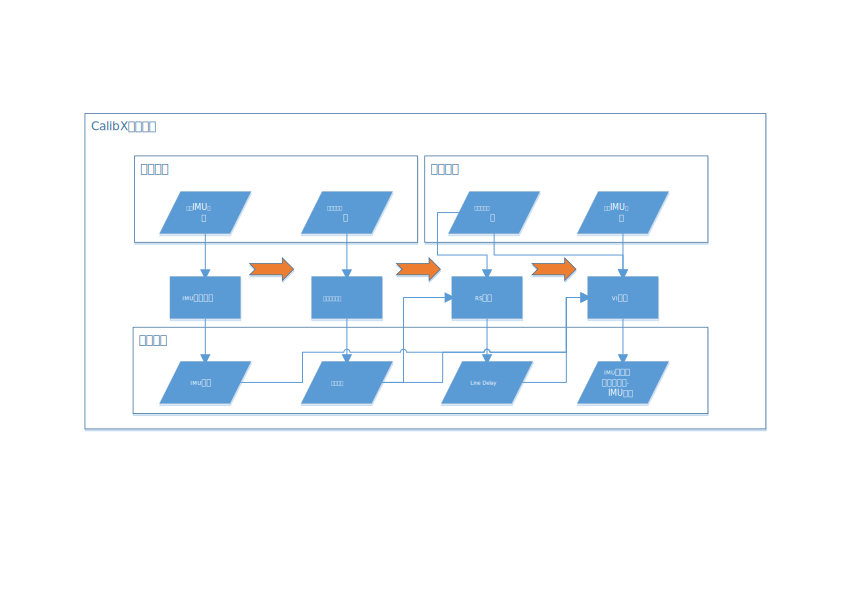
\includegraphics[width=1\textwidth]{figure/cp10/calibx_framework}
	\caption{CalibX硬件系统}
	\label{fig:calibx_framework}
\end{figure}
目前支持3种相机模型:
\begin{itemize}
	\item Pinhole-brown和pinhole-radtan。主要面向小畸变、小视场角(FOV)的相机。
	\item Pinhole-equidistant。主要面向大畸变、大视场角的相机(FOV $\le $ 180°),主要是广角相机和鱼眼相机。
\end{itemize}
支持4种标定板,如图\ref{fig:calibx-calibration-board}所示。:
\begin{itemize}
	\item 棋盘格。
	\item CircleGrid。
	\item Apriltag。
	\item RandomGrid。
\end{itemize}
\begin{figure}
	\centering
	\begin{minipage}{0.45\linewidth}
		\centering
		\subfigure[棋盘格]{\includegraphics[width=5cm]{figure/cp10/chessboard}}
		\label{fig:chessboard}
	\end{minipage}\qquad
	\begin{minipage}{0.45\linewidth}
		\centering
		\subfigure[CircleGrid]{\includegraphics[width=5cm]{figure/cp10/circlegrid}}
		\label{fig:circlegrid}
	\end{minipage}
	\begin{minipage}{0.45\linewidth}
		\centering
		\subfigure[Apriltag]{\includegraphics[width=5cm]{figure/cp10/apriltag}}
		\label{fig:apriltag}
	\end{minipage}\qquad
	\begin{minipage}{0.45\linewidth}
		\centering
		\subfigure[RandomGrid]{\includegraphics[width=5cm]{figure/cp10/randomgrid}}
		\label{fig:randomgrid}
	\end{minipage}
	\caption{CalibX标定系统支持的标定板}
	\label{fig:calibx-calibration-board}
\end{figure}
其中,棋盘格和CircleGrid为无局部编码的标定板,Apriltag和RandomGrid为局部编码标定板。\\
CalibX总结有如下优点:
\begin{itemize}
	\item 支持多种相机模型,覆盖普通相机、广角相机和鱼眼相机。
	\item 支持多种类型标定板,支持多块同一类型的、局部编码标定板。比如3块RandomGrid构成的立体直角。
	\item 支持多相机,多相机允许是不同类型相机的组合,如普通相机和鱼眼相机、卷帘曝光相机和全局曝光相机。多相机标定支持重叠视场和无重叠视场两种类型。
	\item 标定速度快。静态标定仅用几张图就能完成标定,标定时间不超过30s。RS标定和联标总计在5分钟内完成。
	\item 高精度。正常情况下,多相机标定基线与设计值的误差在1mm以内,相机与IMU外参平移误差在3mm以内\footnote{标定设备是OPPO无面罩AR眼镜\label{calibration_device}}。
	\item 高重复性精度。与市面上在售的产品\cite{indemind}相比,相机与IMU外参旋转角重复性精度高10倍\textsuperscript{\ref{calibration_device}}!如表\ref{tab:calibx-vs-indemind}所示。
\end{itemize}
\begin{table*}[t]
	\centering
	\caption{CalibX与Indemind标定对比}
	\label{tab:calibx-vs-indemind}
	\begin{tabular}{|c|c|c|c|c|}
		\hline
		方案 & 组别 &  Yaw/° & Pitch/° & Roll/° \\
		\hline
		\multirow{4}{*}{Indemind-双目模组} &1 & -179.521225 & -0.439943 & 0.622170 \\
		\cline{2-5}
		\multirow{4}{*}{} & 2 &-179.602241	&-0.463838	&0.598827 \\
		\cline{2-5}
		\multirow{4}{*}{} & 3 &-179.780491	&-0.662679	&0.404572 \\
		\cline{2-5}
		\multirow{4}{*}{} & STD &0.1326	&0.1223	&0.1195 \\
		\cline{2-5}
		\hline
		\multirow{4}{*}{CalibX-OPPO眼镜} &1 & -89.940266 & 0.209434 & 179.883943 \\
		\cline{2-5}
		\multirow{4}{*}{} & 2 &-89.926987	&0.231154	&179.889317 \\
		\cline{2-5}
		\multirow{4}{*}{} & 3 &-89.919383	&0.258630	&179.889180 \\
		\cline{2-5}
		\multirow{4}{*}{} & STD &0.0106	&0.0247	&0.0031 \\
		\cline{2-5}
		\hline
	\end{tabular}
\end{table*}
